\documentclass[../main.tex]{subfiles}

\graphicspath{{\subfix{../figures/}}}

\begin{document}

\gls{cryoem} is an image acquisition technique that uses \glspl{tem} to examine a frozen sample. Unlike traditional optical microscopes, \glspl{tem} use a electron beam instead of light, which allows them to capture images at much higher resolution. As a consequence, it has become a very popular technique for collecting images of biological molecules, such as proteins\cite{chemistry_world_cryoem}.

However, \glspl{tem} require very specific conditions in order to work, such as a near perfect vacuum and high-energy electrons. Therefore, they are unsuitable for biological samples, as these are too fragile to endure in such conditions. Here is where the cryogenic part comes into place. In order to retain the sample intact and in place, a thin film of ice is used. The sample is cooled down very rapidly, so that the water has no time to form an ice lattice, avoiding the diffraction of the electron beam. This technique was awarded with the 2017 Nobel Prize in Chemistry\cite{chemistry_world_cryoem}.

\begin{figure}[htbp]
    \centering
    \begin{subfigure}[b]{0.3\textwidth}
         \centering
         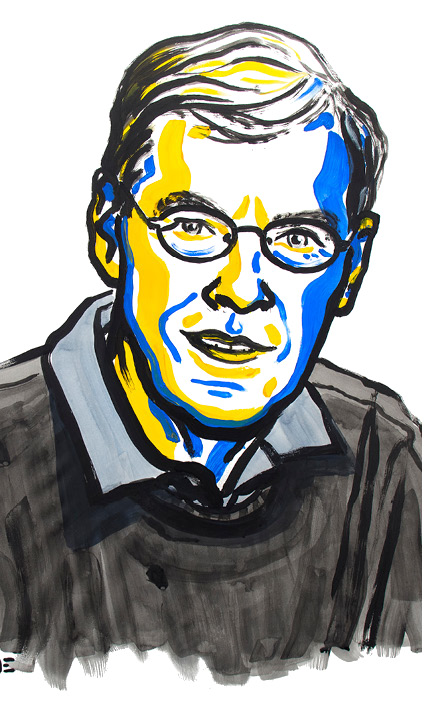
\includegraphics[width=\textwidth]{nobel2017/Richard Henderson}
         \caption{Richard Henderson}
         \label{fig:1:nobel2017:richard}
    \end{subfigure}
    \hfill
    \begin{subfigure}[b]{0.3\textwidth}
         \centering
         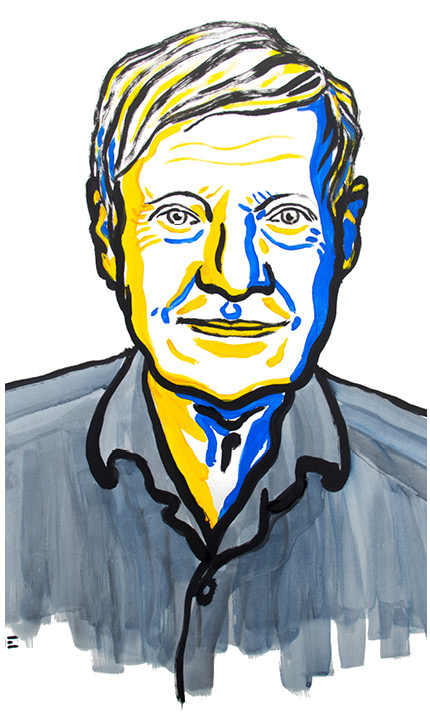
\includegraphics[width=\textwidth]{nobel2017/Joachim Frank}
         \caption{Joachim Frank}
         \label{fig:1:nobel2017:joachim}
    \end{subfigure}
    \hfill
    \begin{subfigure}[b]{0.3\textwidth}
         \centering
         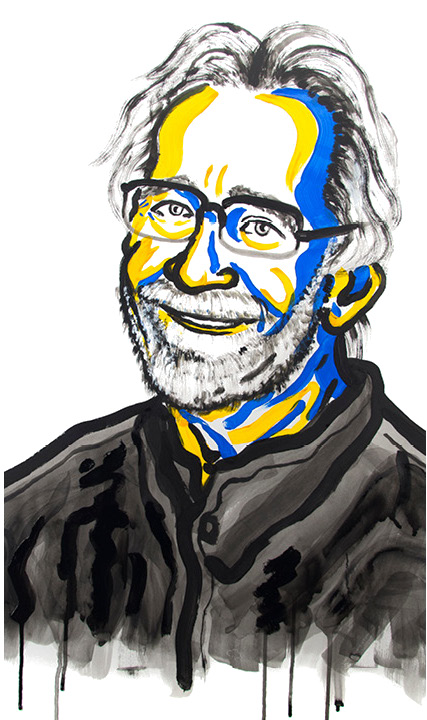
\includegraphics[width=\textwidth]{nobel2017/Jacques Dubochet}
         \caption{Jacques Dubochet}
         \label{fig:1:nobel2017:jaques}
    \end{subfigure}\\
    Images obtained from: \cite{science_nobel}
    \caption{2017 Nobel Prize in Chemistry}
    \label{fig:1:nobel2017}
\end{figure}

Usually, the sample is prepared on a copper or gold grid, which may hold thousands of specimens under study, each of them with a random orientation. Each of these specimens is known as ``particle''. Assuming that all particles belong to the same structure, their 2D projections can be used to mathematically infer the 3D structure of the specimen\cite{cryoem101}. \Gls{spa} is a family of image acquisition and processing techniques that enables such a task.

At the beginning of the \gls{spa} image processing pipeline, a large quantity of noisy data is provided, from which little to no parameters are known. Therefore, all of the parameters needed for reconstruction must be estimated from the data. The projection direction of each of the particles is among the unknowns. The process of deducing their orientation is known as 3D particle alignment, which will be the focus of this work.

This project has been carried out at the Biocomputing Unit of \gls{cnb}-\gls{csic}, located in Madrid. This research group develops two software suites related to \gls{cryoem}, Xmipp and Scipion. The former one implements image processing algorithms, whilst the later one provides a framework to easily interoperate between current image processing suites.

The aim of this project is to develop a fast \gls{gpu} accelerated computer program to align particles. The key innovation of this project is the usage of state-of-the-art vector search databases. This software will be implemented inside Xmipp and it will be integrated into Scipion.

\section{Objectives}
The main objective of this thesis is to develop a fast and accurate image alignment algorithm for \gls{cryoem}. To be more precise, the algorithm will focus on performing 3D alignments of particles, this is, it will be used to deduce their orientation. Nevertheless, it will leave room for its application in other image alignment problems in \gls{cryoem}.

In general, the image alignment problem involves finding the best match for an image across a large set of images, also considering their rotations and shifts. As a consequence, this process involves comparing many image pairs, making it computationally expensive. In addition, it is a recurrent problem in the context of \gls{spa} and other \gls{cryoem} image processing techniques.

This means that current image processing workflows dedicate a large amount of time and resources to run this type of algorithms. Reducing image alignment times significantly reduces the computation time required to solve a protein structure. This performance improvement involves several benefits. Firstly, it allows to make more efficient use of the available computational resources, which may be scarce due to the cost associated to high-end workstations and servers. Moreover, a higher throughput can be achieved, enabling to reach further results in streaming. Last but not least, biologist are able to deduce conclusions and iterate must faster, accelerating drug and vaccine developments.

Similarly, this widespread usage of alignment processes in \gls{cryoem} also implies that the quality of the final results is heavily influenced by their accuracy.

These facts have motivated the development of a new image alignment algorithm that tries to maximise throughput at little accuracy cost. The base idea is to use novel vector compression techniques to accelerate searches. Similarly to state-of-the-art alignment algorithms, our algorithm should also run on \gls{gpu} accelerators, as these are very suitable for image processing tasks, offering orders of magnitude more compute power than \glspl{cpu}.

One of the current developments in the context of \gls{spa} is the ability to run streaming workflows. This means that data is processed in the same pace that it is generated in the microscope. Therefore, a certain performance level is required to keep up with the data acquisition. Streaming workflows allow to obtain results earlier and provide feedback to the microscope. This allows to operate the microscope in a semi-automatic and effective manner, leading to an optimal utilisation of it.

Consequently, another pursued innovation of this project is the ability to run in streaming workflows. In other words, the algorithm should be able to run in real-time provided that reasonable hardware is available to it. This would mean that refinements beyond initial volumes could be achieved in streaming, which none of the current processing suits is able to.

\section{Structure of the document}
TO BE COMPLETED

\end{document}
 